% Created 2020-08-04 ter 14:57
% Intended LaTeX compiler: pdflatex
\documentclass[17pt, a4paper]{extarticle}
\usepackage[utf8]{inputenc}
\usepackage[T1]{fontenc}
\usepackage{graphicx}
\usepackage{grffile}
\usepackage{longtable}
\usepackage{wrapfig}
\usepackage{rotating}
\usepackage[normalem]{ulem}
\usepackage{amsmath}
\usepackage{textcomp}
\usepackage{tikz}
\usepackage{mathdots}
\usepackage{cancel}
\usepackage{color}
\usepackage{array}
\usepackage{multirow}
\usepackage{amssymb}
\usepackage{gensymb}
\usepackage{tabularx}
\usepackage{booktabs}
\usetikzlibrary{fadings}
\usetikzlibrary{patterns}
\usetikzlibrary{shapes}
\usepackage{amssymb}
\usepackage{tgbonum}
\usepackage{capt-of}
\usepackage{hyperref}
\usepackage{pdfpages}
\hypersetup{pdfborder = {0 0 0}}
\usepackage{graphicx}
\setlength{\parskip}{\baselineskip}
\usepackage{indentfirst}
\author{Biel A. P.}
\date{2020}
\title{An Introduction to Software Reverse Engineering.}
\begin{document}

%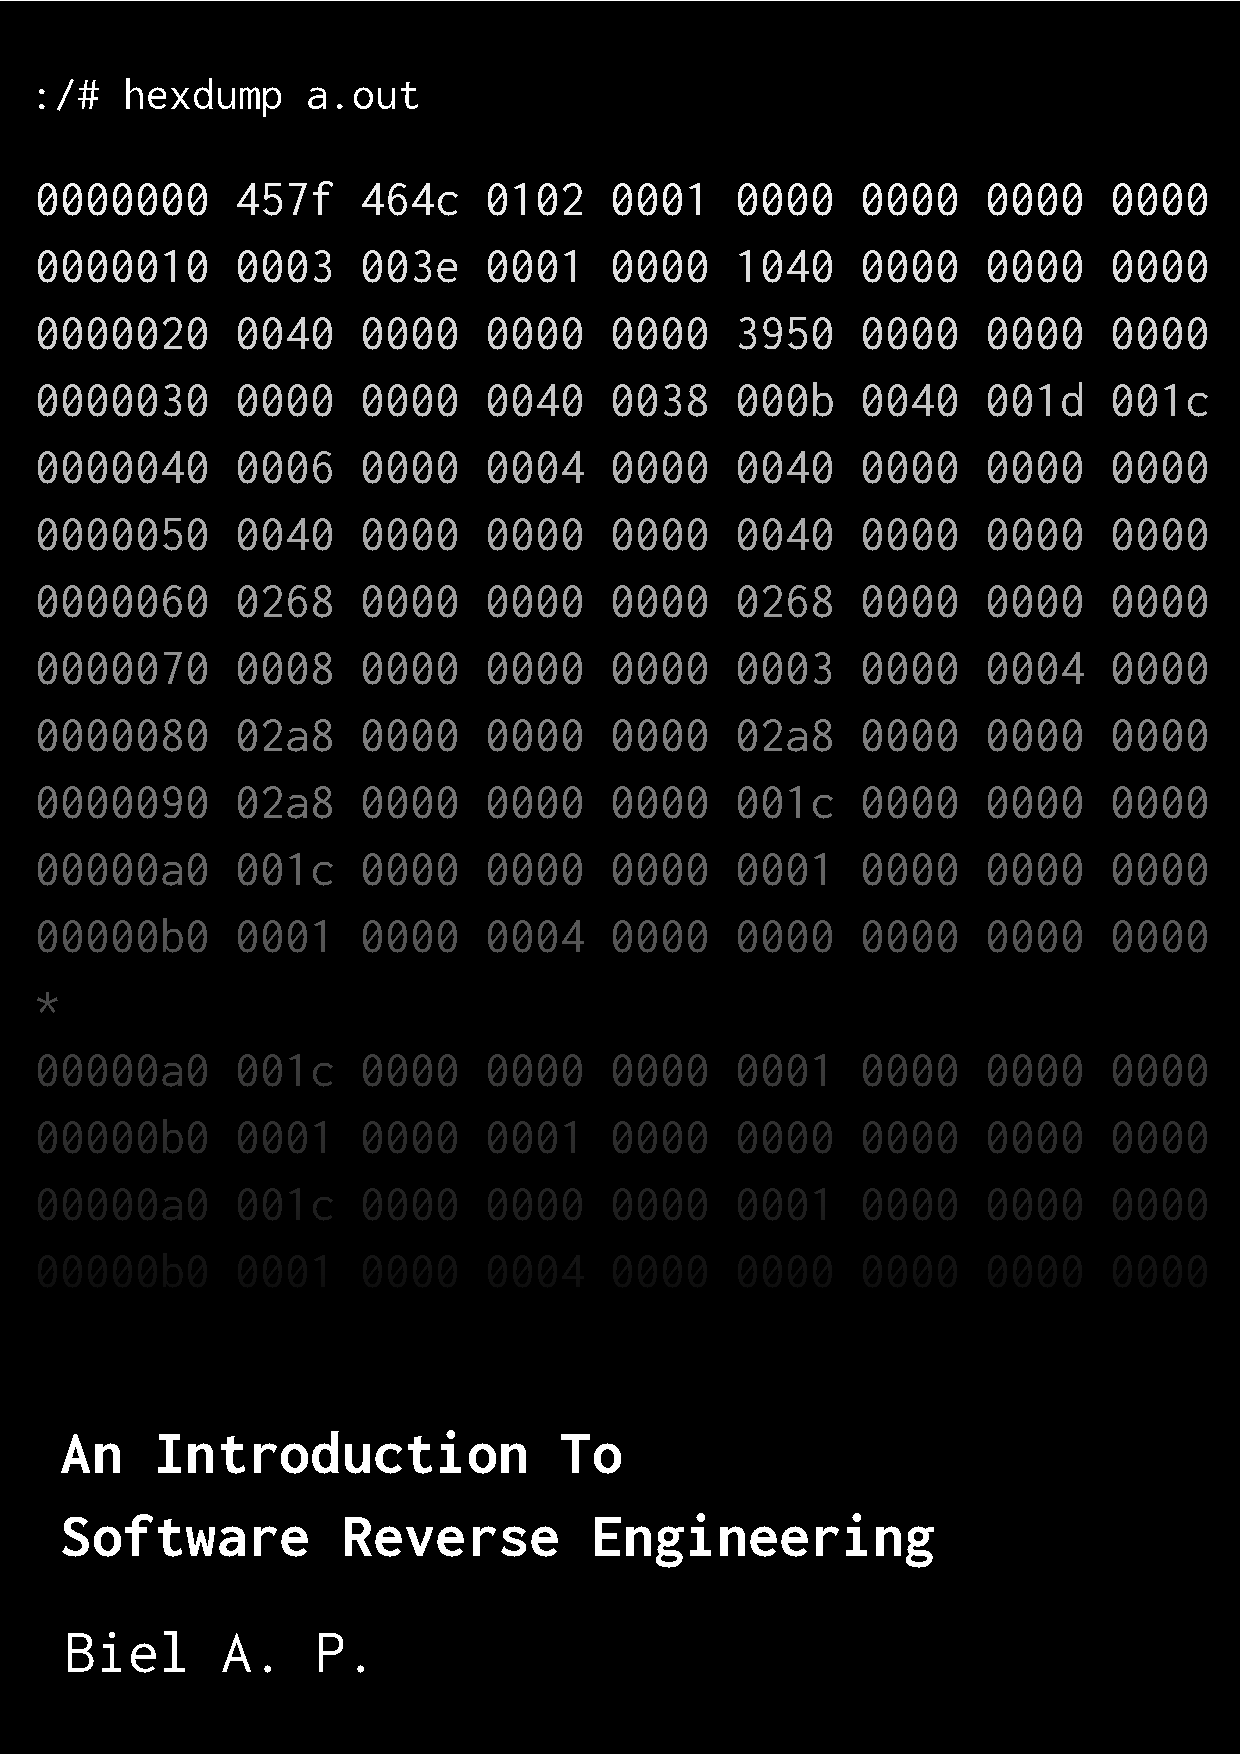
\includepdf[pages=1, fitpaper]{coverpage}
\maketitle
\newpage

\tableofcontents
\newpage

\section{Introduction}

Hi, Welcome! My name's Biel and I'm a Cyber Security Analyst. I'm writing this book with the goal to introduce reverse engineering to people who has the interest in it but doesn't know where to start. It is assumed that the readers already have programming experience, if not, this book may not be for you at the moment. 

We will talk about files, binary files, PE, ELF, and a lot of other reverse engineering related subjects so people who have never had contact with reverse engineering can start doing it.

During the book, the software I'm using is:

\begin{itemize}
\item OS: Arch Linux;
\item Shell: Bash;
\item Dumpers: objdump, hexdump;
\item Text Editor: VIM;
\item Hex Editor: hx;
\item Tracers: ltrace, strace;
\item Disassembler: radare2;
\end{itemize}

But feel free to use the software you are used to, I use those because they are free and Open Source but I won't try to convert you to the Open Source\ldots{} Maybe on my next book\ldots{}

\newpage

\section{Files}
\subsection{What is a file?}

In short, a file is a sequence of binaries stored somewhere that is referenced by another element. The minimum size something has to have to be considered a file, is 1 byte, or 8 bits, or 10101010 and it can be anything, a text file, an audio file, an executable file, anything, as long as it has 1 byte.

\subsection{How a file become a file?}

So, as you learnt, a file is something with at least 1 byte, 1 byte in binary code is \textit{10101010}, but how does this works? how the computer understands this?

Let's imagine you wrote a program in \textbf{C}, that is what happens behind the scenes when you compile the program:



\tikzset{every picture/.style={line width=0.75pt}} %set default line width to 0.75pt

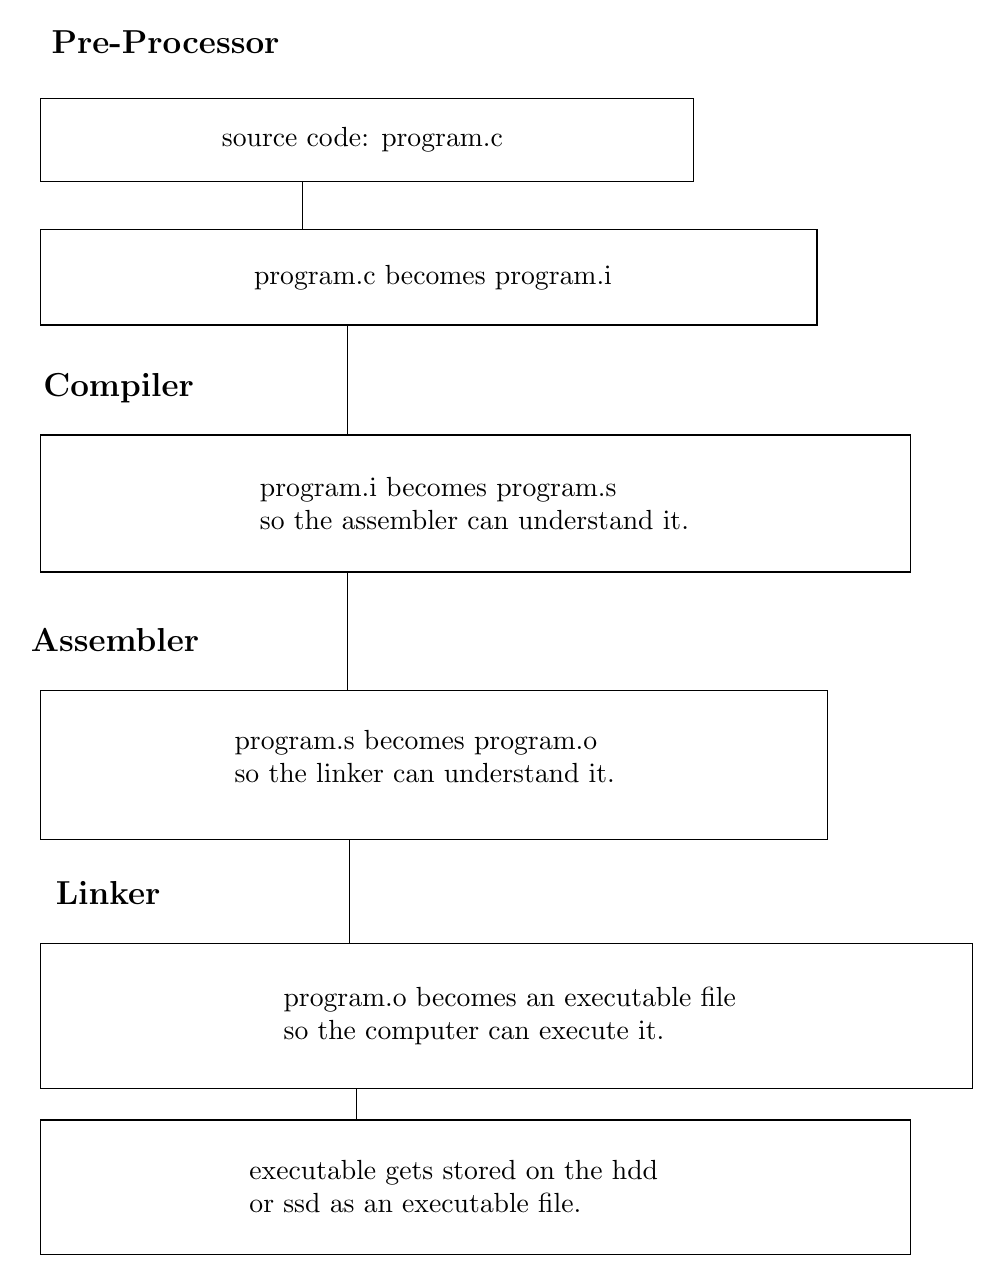
\begin{tikzpicture}[x=0.75pt,y=0.75pt,yscale=-1,xscale=1]
%uncomment if require: \path (0,632); %set diagram left start at 0, and has height of 632

%Straight Lines [id:da5153810176025947]
\draw    (149,128) -- (149,240) ;
%Straight Lines [id:da906378895835927]
\draw    (127,76) -- (127,135) ;
%Shape: Rectangle [id:dp8428256722279753]
\draw  [color={rgb, 255:red, 0; green, 0; blue, 0 }  ,draw opacity=1 ][fill={rgb, 255:red, 255; green, 255; blue, 255 }  ,fill opacity=1 ] (1,43) -- (315.5,43) -- (315.5,83) -- (1,83) -- cycle ;
%Shape: Rectangle [id:dp5611969127012603]
\draw  [color={rgb, 255:red, 0; green, 0; blue, 0 }  ,draw opacity=1 ][fill={rgb, 255:red, 255; green, 255; blue, 255 }  ,fill opacity=1 ] (1,106) -- (375,106) -- (375,152) -- (1,152) -- cycle ;
%Shape: Rectangle [id:dp746632881475329]
\draw  [color={rgb, 255:red, 0; green, 0; blue, 0 }  ,draw opacity=1 ][fill={rgb, 255:red, 255; green, 255; blue, 255 }  ,fill opacity=1 ] (1,205) -- (420,205) -- (420,271) -- (1,271) -- cycle ;
%Straight Lines [id:da6780542717486732]
\draw    (149,271) -- (149,363) ;
%Shape: Rectangle [id:dp6706740493686194]
\draw  [color={rgb, 255:red, 0; green, 0; blue, 0 }  ,draw opacity=1 ][fill={rgb, 255:red, 255; green, 255; blue, 255 }  ,fill opacity=1 ] (1,328) -- (380,328) -- (380,400) -- (1,400) -- cycle ;
%Straight Lines [id:da6001654561119104]
\draw    (150,400) -- (150,485) ;
%Shape: Rectangle [id:dp5601860311201697]
\draw  [color={rgb, 255:red, 0; green, 0; blue, 0 }  ,draw opacity=1 ][fill={rgb, 255:red, 255; green, 255; blue, 255 }  ,fill opacity=1 ] (1,450) -- (450,450) -- (450,520) -- (1,520) -- cycle ;
%Straight Lines [id:da3479082266811051]
\draw    (153,520) -- (153,554) ;
%Shape: Rectangle [id:dp06774102179156838]
\draw  [color={rgb, 255:red, 0; green, 0; blue, 0 }  ,draw opacity=1 ][fill={rgb, 255:red, 255; green, 255; blue, 255 }  ,fill opacity=1 ] (1,535) -- (420,535) -- (420,600) -- (1,600) -- cycle ;

% Text Node
\draw (156,62.5) node   [align=center] {source code: program.c};
% Text Node
\draw (5,9) node [anchor=north west][inner sep=0.75pt]   [align=left] {\textbf{{\large Pre-Processor}}};
% Text Node
\draw (190,129) node   [align=center] {program.c becomes program.i};
% Text Node
\draw (210,238) node   [align=left] {program.i becomes program.s\\so the assembler can understand it.};
% Text Node
\draw (1,174) node [anchor=north west][inner sep=0.75pt]   [align=left] {\textbf{{\large Compiler}}};
% Text Node
\draw (186,360) node   [align=left] {program.s becomes program.o\\so the linker can understand it.};
% Text Node
\draw (-5,297) node [anchor=north west][inner sep=0.75pt]   [align=left] {\textbf{{\large Assembler}}};
% Text Node
\draw (227,485) node   [align=left] {program.o becomes an executable file\\so the computer can execute it.};
% Text Node
\draw (7,419) node [anchor=north west][inner sep=0.75pt]   [align=left] {\textbf{{\large Linker}}};
% Text Node
\draw (200,567) node   [align=left] {executable gets stored on the hdd\\or ssd as an executable file.};


\end{tikzpicture}

After that, the program is ready for execution, depending on the hardware and the programming language you are using, this process can be slower or faster. Usually low level programming languages such as \textbf{Assembly} and \textbf{C} compile faster than high level programming languages such as \textbf{Python} and \textbf{Java}.

\subsection{How a program is executed?}

Basically, after the program is stored on the hard drive or solid state drive, it becomes a process on the computer. This process go through a \textbf{loader} and gets allocated on the \textbf{Process Address Space}, usually on the \textbf{RAM}.

\tikzset{every picture/.style={line width=0.75pt}} %set default line width to 0.75pt

\begin{tikzpicture}[x=0.75pt,y=0.75pt,yscale=-1,xscale=1]
%uncomment if require: \path (0,632); %set diagram left start at 0, and has height of 632

%Shape: Rectangle [id:dp06774102179156838]
\draw  [color={rgb, 255:red, 0; green, 0; blue, 0 }  ,draw opacity=1 ][fill={rgb, 255:red, 255; green, 255; blue, 255 }  ,fill opacity=1 ] (1,535) -- (420,535) -- (420,600) -- (1,600) -- cycle ;

%Straight Lines [id:da3479082266811051]
\draw    (153,700) -- (153,600) ;

%Shape: Rectangle [id:dp06774102179156838]
\draw  [color={rgb, 255:red, 0; green, 0; blue, 0 }  ,draw opacity=1 ][fill={rgb, 255:red, 255; green, 255; blue, 255 }  ,fill opacity=1 ] (1,835) -- (420,835) -- (420,700) -- (1,700) -- cycle ;


% Text Node
\draw (7,500) node [anchor=north west][inner sep=0.75pt]   [align=left] {\textbf{{\large Loader}}};

% Text Node
\draw (200,567) node   [align=left] {stored executable.};

% Text Node
\draw (210,767) node   [align=left] {\textbf{{\large Process Address Space.}}};


\end{tikzpicture}


\end{document}
